\section{条件梯度法（Frank--Wolfe）}
\label{sec:feas-fw}

投影的代价可能很高，而同一个集合上的线性函数却容易最小化。能不能完全不做投影，只靠线性最小化来保持可行？本节回答这个问题：\term{条件梯度法}（conditional gradient method）也称\term{Frank--Wolfe法}（Frank--Wolfe method）\scite{frank1956algorithm}，它要求集合紧，用目标的一阶信息挑选集合的极点，再用凸组合保持可行。

\paragraph{主要思想}
把目标在当前点线性化，$f(\bm{x})+\langle\bm{g},\bm{s}-\bm{x}\rangle$。线性模型没有碗底，无约束时可以降到负无穷，这正是梯度下降要加二次项的原因。现在集合是紧的，线性模型在集合上有最小点，所以可以直接问：只信线性模型的话，集合里哪个点最好？

这个点$\bm{s}^{(t)}$通常在集合的远端，线性模型不能信到那么远。于是不跳过去，只沿连线走一段：
\begin{equation}
 \begin{aligned}
 \bm{s}^{(t)}&\in\argmin_{\bm{s}\in\bm{C}}\langle\bm{g}^{(t)},\bm{s}\rangle,\\
 \bm{x}^{(t+1)}&=\bm{x}^{(t)}+\alpha^{(t)}\bigl(\bm{s}^{(t)}-\bm{x}^{(t)}\bigr),\quad\alpha^{(t)}\in[0,1].
 \end{aligned}
 \label{eq:feas-fw}
\end{equation}

新点是两个可行点的凸组合，所以可行性由$\alpha^{(t)}\in[0,1]$和$\bm{C}$的凸性保证，不需要任何拉回操作。两种方法的次序相反：投影梯度先走一小步再修正，条件梯度先选定目标位置，再决定走多远。

\subsection{线性子问题}
\label{sec:feas-fw-linear}

式~\eqref{eq:feas-fw}的第一行要解一个线性规划。在单纯形上它有闭式解，并且解的形状决定了迭代点的结构。

\paragraph{单纯形上的线性最小化}
对任意$\bm{s}\in\bm{\Delta}$，$\bm{s}$的坐标非负且和为一，$\langle\bm{g},\bm{s}\rangle$是$g_i$的加权平均，所以
\[
 \langle\bm{g},\bm{s}\rangle=\sum_is_ig_i\geq\min_ig_i.
\]
等号在把全部权重放到最小坐标上时取得。因此线性子问题的一个解是顶点
\begin{equation}
 \bm{s}=\bm{e}_{i},\qquad i\in\argmin_kg_k.
 \label{eq:feas-simplex-lmo}
\end{equation}
只需找出梯度的最小分量，计算量是$O(n)$，不用排序。

这个结论在任何紧凸集上都有对应：线性函数的最小值总可以在极点处取到。所以线性子问题的解是集合中结构最简单的点。例如迹为一的半正定矩阵集合的极点是秩一矩阵，线性子问题的解就是$\bm{v}\bm{v}^\top$，其中$\bm{v}$是梯度矩阵最小特征值的单位特征向量。

\paragraph{稀疏表示}
每轮新点等于旧点乘以$1-\alpha^{(t)}$，再给选中的顶点加上权重$\alpha^{(t)}$。若把$\bm{x}^{(t)}$写成顶点的凸组合，权重的更新就是
\begin{equation}
 w_{v}\leftarrow(1-\alpha^{(t)})w_{v},\quad v\neq i;
 \qquad
 w_{i}\leftarrow(1-\alpha^{(t)})w_{i}+\alpha^{(t)}.
 \label{eq:feas-fw-weights}
\end{equation}

从一个顶点出发，每轮至多引入一个新顶点，所以$\bm{x}^{(t)}$至多是$t+1$个顶点的组合。在单纯形上这意味着至多有$t+1$个非零坐标。旧顶点的权重只被等比例缩小，这一点后面会成为问题。

\needspace{6\baselineskip}
\paragraph{变量}
\begin{itemize}
 \item $\bm{x}^{(t)}\in\bm{C}$：当前点；$\bm{g}^{(t)}$：当前梯度。
 \item $\bm{s}^{(t)}\in\bm{C}$：线性子问题的解，这里是顶点。
 \item $w_v$：各活跃顶点的权重，只在需要稀疏表示时保存。
 \item $\alpha^{(t)}\in[0,1]$：组合系数。
\end{itemize}

\paragraph{初始化}
选一个可行点，通常是一个顶点，令$t=0$。例中取$\bm{x}^{(0)}=\bm{e}_3=(0,0,1)$，目标值$f(\bm{x}^{(0)})=2.28125$，组合系数取预定序列
\begin{equation}
 \alpha^{(t)}=\frac{2}{t+2}.
 \label{eq:feas-fw-open-step}
\end{equation}

\needspace{6\baselineskip}
\paragraph{每轮更新}
在第$t$轮：
\begin{enumerate}
 \item \textbf{解线性子问题。}由式~\eqref{eq:feas-simplex-lmo}选顶点。例中第一轮
 \[
  \bm{g}^{(0)}=(-1,-2.5,2),\qquad \bm{s}^{(0)}=\bm{e}_2.
 \]
 \item \textbf{组合。}由式~\eqref{eq:feas-fw}计算新点。例中第一轮$\alpha^{(0)}=1$，新点直接跳到顶点，$\bm{e}_3$的权重变成零：
 \[
  \bm{x}^{(1)}=(0,1,0),\qquad f(\bm{x}^{(1)})=0.78125.
 \]
 \item \textbf{检查停止。}若$t+1=T$，输出$\bm{x}^{(t+1)}$；否则$t\leftarrow t+1$。第~\ref{sec:feas-fw-gap}节会给出可以计算的停止量，例中暂取$T=100$。
\end{enumerate}

例中第二轮，$\bm{g}^{(1)}=(-1,1.5,0)$，选$\bm{e}_1$，$\alpha^{(1)}=\tfrac23$，于是
\[
 \bm{x}^{(2)}=\bigl(\tfrac23,\tfrac13,0\bigr),\qquad f(\bm{x}^{(2)})\approx0.22569.
\]

例中第三轮，$\bm{g}^{(2)}=(-\tfrac13,-\tfrac76,0)$，选$\bm{e}_2$，$\alpha^{(2)}=\tfrac12$，于是
\[
 \bm{x}^{(3)}=\bigl(\tfrac13,\tfrac23,0\bigr),\qquad f(\bm{x}^{(3)})\approx0.22569.
\]

例中第四轮，$\bm{g}^{(3)}=(-\tfrac23,\tfrac16,0)$，选$\bm{e}_1$，$\alpha^{(3)}=\tfrac25$，于是
\[
 \bm{x}^{(4)}=\bigl(\tfrac35,\tfrac25,0\bigr),\qquad f(\bm{x}^{(4)})=0.18125.
\]

规律已经出现：两个顶点轮流被选中，迭代点在解$(\tfrac12,\tfrac12,0)$的两侧来回摆动，幅度慢慢变小。最终在$T=100$得到的点，目标差约为$6.1\times10^{-5}$。

图~\ref{fig:feas-fw-path-weights}画出路径和权重。第一步把起点的权重清零，这是$\alpha^{(0)}=1$的特殊效果。之后的权重在$\bm{e}_1$和$\bm{e}_2$之间来回转移。

\begin{BookInlineFigure}
  \centering
  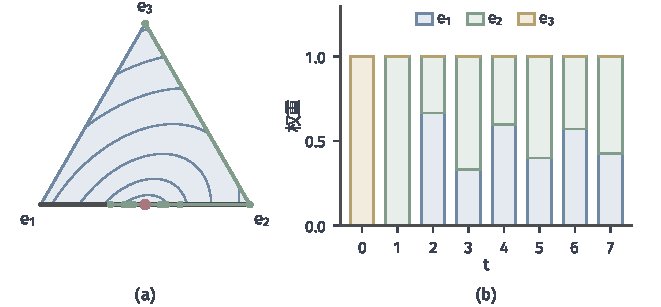
\includegraphics[width=112mm]{figures/05-optimization/06-constrained-optimization/matplotlib/feas-fw-path-weights/figure.pdf}
  \caption{条件梯度法的路径与权重，$\alpha^{(t)}=2/(t+2)$，从顶点$\bm{e}_3$出发。(a)绿色路径先跳到$\bm{e}_2$，然后沿活动边在解（红点）两侧摆动。(b)前$8$个迭代点在三个顶点上的权重，第$t$根柱子的三段高度是$\bm{x}^{(t)}$的三个坐标。}
  \label{fig:feas-fw-path-weights}
\end{BookInlineFigure}

\subsection{步长与可行性}
\label{sec:feas-fw-step}

式~\eqref{eq:feas-fw}中的$\alpha^{(t)}$可以怎样选，不同选法各用到什么信息？

\paragraph{三种规则}
记方向$\bm{d}^{(t)}=\bm{s}^{(t)}-\bm{x}^{(t)}$，用
\begin{equation}
 \Gamma^{(t)}=\langle\bm{g}^{(t)},\bm{x}^{(t)}-\bm{s}^{(t)}\rangle\geq0
 \label{eq:feas-fw-gamma-step}
\end{equation}
表示线性模型沿整条线段预测的下降量。三种规则如下。

\begin{itemize}
 \item \textbf{预定序列。}用式~\eqref{eq:feas-fw-open-step}，不需要函数值，也不需要$L$。
 \item \textbf{线搜索。}$\alpha^{(t)}\in\argmin_{\alpha\in[0,1]}f(\bm{x}^{(t)}+\alpha\bm{d}^{(t)})$，把范围限制在$[0,1]$是为了留在线段上。
 \item \textbf{光滑上界。}最小化下降引理的上界，在$[0,1]$上截断：
\end{itemize}
\begin{equation}
 \alpha^{(t)}=\min\Bigl\{1,\ \frac{\Gamma^{(t)}}{L\lVert\bm{d}^{(t)}\rVert_2^2}\Bigr\}.
 \label{eq:feas-fw-smooth-step}
\end{equation}

三种规则都使$\alpha^{(t)}\in[0,1]$。预定序列在$t\geq0$时取值从$1$递减。线搜索按定义在区间内。光滑上界的分子非负，分母为正（若分母为零，则$\bm{s}^{(t)}=\bm{x}^{(t)}$，已不必移动），再用$\min$截断。

在预算例的第一轮比较这三种规则。方向是$\bm{e}_2-\bm{e}_3=(0,1,-1)$，需要的几个量是
\[
 \Gamma^{(0)}=4.5,\qquad \lVert\bm{d}\rVert_2^2=2,\qquad \bm{d}^\top\bm{H}\bm{d}=6.
\]

二次目标上的精确线搜索是$\Gamma/(\bm{d}^\top\bm{H}\bm{d})$，所以
\[
 \alpha_{\text{预定}}=1,\qquad
 \alpha_{\text{线搜索}}=\tfrac34,\qquad
 \alpha_{\text{上界}}=\tfrac{9}{16}.
\]

对应的目标值分别是$0.78125$、$0.59375$和$0.69922$，图~\ref{fig:feas-fw-step-rules}(a)把这三点标在沿线段的目标曲线上。

\begin{BookInlineFigure}
  \centering
  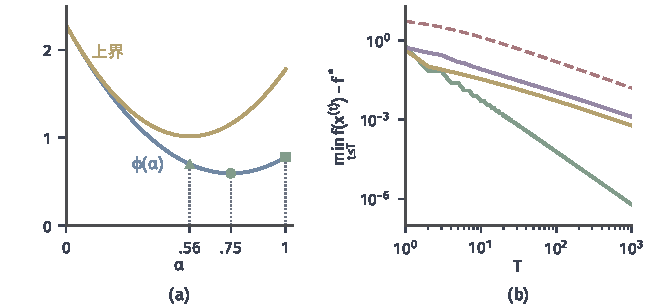
\includegraphics[width=112mm]{figures/05-optimization/06-constrained-optimization/matplotlib/feas-fw-step-rules/figure.pdf}
  \caption{组合系数的三种选法。(a)蓝线是从$\bm{e}_3$到$\bm{e}_2$的线段上的目标$\phi(\alpha)$，黄线是光滑上界，三角、圆点、方块分别是光滑上界、线搜索、预定序列对应的系数。(b)迄今最小目标差：绿线是预定序列，黄线是线搜索，紫线是光滑上界，红色虚线是定理~\ref{thm:feas-fw-rate}的上界$16/(T+2)$。}
  \label{fig:feas-fw-step-rules}
\end{BookInlineFigure}

\paragraph{有限步界}
下面证明目标差的上界，同时把线性子问题解得不准的情形放进去。设$\bm{C}$的直径是$D$，即集合中两点欧氏距离的最大值。证明要用到下一小节将要单独研究的一个事实，这里先在证明中直接用凸性得到。

\begin{theorem}[条件梯度法的有限步界]
\label{thm:feas-fw-rate}
设$\bm{C}$非空紧凸，直径为$D$，$f$在包含$\bm{C}$的开集上可微，在$\bm{C}$上凸且$L$光滑，$\delta\geq0$。设线性子问题的解$\tilde{\bm{s}}^{(t)}\in\bm{C}$满足
\begin{equation}
 \langle\bm{g}^{(t)},\tilde{\bm{s}}^{(t)}\rangle\leq\min_{\bm{s}\in\bm{C}}\langle\bm{g}^{(t)},\bm{s}\rangle+\frac{\delta}{2}\alpha^{(t)}LD^2,
 \label{eq:feas-inexact-lmo}
\end{equation}
并取$\alpha^{(t)}=2/(t+2)$。则对$T\geq1$，
\begin{equation}
 f(\bm{x}^{(T)})-f^\star\leq\frac{2(1+\delta)LD^2}{T+2}.
 \label{eq:feas-fw-rate}
\end{equation}
\end{theorem}

\begin{proof}
记$e_t=f(\bm{x}^{(t)})-f^\star$，$\alpha=\alpha^{(t)}$，$\bm{s}^\ast$是线性子问题的精确解。由下降引理，并用直径$D$放大移动的长度，得到
\[
 e_{t+1}\leq e_t+\alpha\langle\bm{g}^{(t)},\tilde{\bm{s}}^{(t)}-\bm{x}^{(t)}\rangle+\frac{L\alpha^2D^2}{2}.
\]

由式~\eqref{eq:feas-inexact-lmo}，把内积中的$\tilde{\bm{s}}^{(t)}$换成$\bm{s}^\ast$：
\[
 e_{t+1}\leq e_t+\alpha\langle\bm{g}^{(t)},\bm{s}^\ast-\bm{x}^{(t)}\rangle+\frac{(1+\delta)L\alpha^2D^2}{2}.
\]

由凸性，切平面在解处不高于目标，再由$\bm{s}^\ast$在线性模型上最优，得到
\[
 \langle\bm{g}^{(t)},\bm{s}^\ast-\bm{x}^{(t)}\rangle\leq\langle\bm{g}^{(t)},\bm{x}^\star-\bm{x}^{(t)}\rangle\leq-e_t.
\]

记$K=(1+\delta)LD^2$，于是得到递推
\[
 e_{t+1}\leq(1-\alpha^{(t)})e_t+\frac{K(\alpha^{(t)})^2}{2}.
\]

下面对$T$归纳证明$e_T\leq2K/(T+2)$。$t=0$时$\alpha^{(0)}=1$，递推给出$e_1\leq K/2\leq2K/3$。设$e_t\leq2K/(t+2)$，$t\geq1$，代入$\alpha^{(t)}=2/(t+2)$：
\[
 e_{t+1}\leq\frac{t}{t+2}\cdot\frac{2K}{t+2}+\frac{2K}{(t+2)^2}=\frac{2K(t+1)}{(t+2)^2}.
\]

由$(t+1)(t+3)\leq(t+2)^2$，右端不超过$2K/(t+3)$，归纳完成。
\end{proof}

$\delta$的作用是把内层误差与外层步长联系起来：式~\eqref{eq:feas-inexact-lmo}允许的误差随$\alpha^{(t)}$减小，也就是越到后面线性子问题要解得越准。如果误差固定不变，递推中多出常数项$\alpha^{(t)}\varepsilon$，目标差最终停在$\varepsilon$的量级。

线搜索和光滑上界的步长满足同样的上界。两者的新点都不高于在$\alpha=2/(t+2)$处的上界值，所以$\delta=0$时递推不变。第一轮的比较也说明，线搜索每步下降最多，并不代表后面的路径更好：图~\ref{fig:feas-fw-step-rules}(b)中，预定序列在这个例子上反而最快，第~\ref{sec:feas-fw-away}节解释其中的原因。

预算例中$D^2=2$，$L=4$，界~\eqref{eq:feas-fw-rate}是$16/(T+2)$，$T=100$时约为$0.157$，实际目标差约$6\times10^{-5}$。这个界对所有满足条件的问题都成立，所以偏于保守。线搜索的黄线大致按$1/T$下降：解在多面体的边上而不是顶点时，线搜索版本的目标差一般不能比$1/T$快多少，证明需要构造性的下界分析，篇幅较长，读者可查阅Frank--Wolfe方法收敛下界的专门文献。预定序列的绿线约按$1/T^2$下降，这来自两个顶点在解的两侧交替抵消的特殊结构，定理并不提供这样的保证。

\subsection{Frank--Wolfe间隙}
\label{sec:feas-fw-gap}

投影梯度用残差判断停止。条件梯度能不能在不知道$f^\star$的情况下，判断离最优还有多远？线性子问题已经算出了答案。

\paragraph{定义与上界}
式~\eqref{eq:feas-fw-gamma-step}的量可以对任意可行点定义。

\begin{definition}[Frank--Wolfe间隙]
\label{def:feas-fw-gap}
设$\bm{C}$非空紧凸，$f$在$\bm{x}\in\bm{C}$处可微，称
\begin{equation}
 \Gamma(\bm{x})=\max_{\bm{s}\in\bm{C}}\langle\nabla f(\bm{x}),\bm{x}-\bm{s}\rangle
 \label{eq:feas-fw-gap}
\end{equation}
为\term{Frank--Wolfe间隙}（Frank--Wolfe gap）。
\end{definition}

取$\bm{s}=\bm{x}$可知$\Gamma(\bm{x})\geq0$。它的值就是线性子问题的副产品，不需要额外计算：式~\eqref{eq:feas-fw-gamma-step}的$\Gamma^{(t)}$正是$\Gamma(\bm{x}^{(t)})$。

这里没有沿用字母$g$，因为$\bm{g}^{(t)}$已经表示梯度。

\begin{theorem}[间隙上界目标差]
\label{thm:feas-fw-gap}
在定义~\ref{def:feas-fw-gap}的条件下，$\Gamma(\bm{x})=0$当且仅当$\bm{x}$满足变分不等式~\eqref{eq:feas-vi}。若$f$在$\bm{C}$上凸，则
\begin{equation}
 f(\bm{x})-\min_{\bm{C}}f\leq\Gamma(\bm{x}).
 \label{eq:feas-fw-gap-bound}
\end{equation}
\end{theorem}

\begin{proof}
由式~\eqref{eq:feas-fw-gap}，$\Gamma(\bm{x})=0$就是对所有$\bm{s}\in\bm{C}$，$\langle\nabla f(\bm{x}),\bm{x}-\bm{s}\rangle\leq0$，这正是式~\eqref{eq:feas-vi}。

设$\bm{x}^\star$是最优解，它存在，因为$\bm{C}$紧、$f$连续。由凸性和$\Gamma$的定义，
\[
 f(\bm{x})-f(\bm{x}^\star)\leq\langle\nabla f(\bm{x}),\bm{x}-\bm{x}^\star\rangle\leq\Gamma(\bm{x}).
\]
\end{proof}

图~\ref{fig:feas-fw-gap-tangent}(a)在一元情形说明这个不等式。切线在集合上的最低值位于端点$\bm{s}$，凸函数高于切线，所以最优值高于切线的最低值。切线在当前点的高度是$f(\bm{x})$，$\Gamma$就是这段高度差。这和第~\ref{chap:duality}章用下界判断最优的思路相同，线性化给出了一个可计算的下界
\[
 f(\bm{x})-\Gamma(\bm{x})\leq f^\star.
\]

\begin{BookInlineFigure}
  \centering
  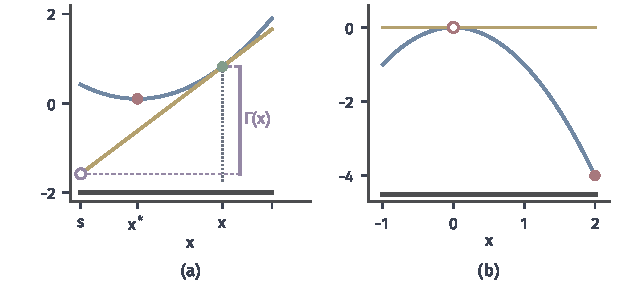
\includegraphics[width=108mm]{figures/05-optimization/06-constrained-optimization/matplotlib/feas-fw-gap-tangent/figure.pdf}
  \caption{间隙的几何。深灰线是可行区间，蓝线是目标，黄线是当前点的切线。(a)凸目标$f(x)=x^2/2+0.1$，$\bm{C}=[-0.8,1.9]$，$x=1.2$：切线在空心紫点处达到区间上的最低值，紫色线段的长度是$\Gamma(x)$，它不小于$f(x)-f^\star$。(b)非凸目标$-x^2$，$\bm{C}=[-1,2]$：局部极大点$x=0$处切线水平，$\Gamma=0$，而全局最优解在$2$。}
  \label{fig:feas-fw-gap-tangent}
\end{BookInlineFigure}

预算例中$\bm{x}^{(3)}=(\tfrac13,\tfrac23,0)$，梯度$(-\tfrac23,\tfrac16,0)$，最小分量是$-\tfrac23$，内积$\langle\bm{g},\bm{x}\rangle=-\tfrac{1}{9}$，于是
\[
 \Gamma(\bm{x}^{(3)})=-\tfrac19+\tfrac23=\tfrac59\approx0.556.
\]
真实目标差约为$0.0694$，不超过间隙。这说明了间隙的特点：可靠但往往偏大。图~\ref{fig:feas-fw-gap-curves}(a)的两条曲线一直保持这种上下关系。

用间隙做停止检验时，可以在每轮计算$\Gamma^{(t)}$，当它不超过容差时输出。把这一步放进第~\ref{sec:feas-fw-linear}节的每轮更新，就得到完整的算法。

\paragraph{非凸目标}
式~\eqref{eq:feas-fw-gap-bound}要用凸性。目标非凸时，$\Gamma=0$只表示一阶驻定，图~\ref{fig:feas-fw-gap-tangent}(b)的局部极大点就是例子。

不过间隙仍能作为进展的度量。取式~\eqref{eq:feas-fw-smooth-step}的步长，把$\lVert\bm{d}\rVert_2$放大为$D$，当$\Gamma\leq LD^2$时一步至少下降$\Gamma^2/(2LD^2)$，否则至少下降$\Gamma/2$。把这些下降量累加，并用$\Delta=f(\bm{x}^{(0)})-\inf_{\bm{C}}f$作为总额，得到
\begin{equation}
 \min_{0\leq t<T}\Gamma(\bm{x}^{(t)})\leq\max\Bigl\{\sqrt{\frac{2LD^2\Delta}{T}},\ \frac{2\Delta}{T}\Bigr\}.
 \label{eq:feas-fw-nonconvex}
\end{equation}
所以驻定度量以$1/\sqrt{T}$的速度减小，和投影残差~\eqref{eq:feas-pgd-nonconvex}开方之后的阶相同。

\paragraph{近似子问题的停止界}
当线性子问题只能近似求解时，设已知误差上界$\varepsilon$：
\[
 \langle\bm{g},\tilde{\bm{s}}\rangle\leq\min_{\bm{s}\in\bm{C}}\langle\bm{g},\bm{s}\rangle+\varepsilon.
\]
用近似解算出来的量记作
\[
 \tilde\Gamma=\langle\bm{g},\bm{x}-\tilde{\bm{s}}\rangle,
\]
它比真实间隙小。把定义和误差条件代入，得到
\begin{equation}
 \tilde\Gamma\leq\Gamma(\bm{x})\leq\tilde\Gamma+\varepsilon.
 \label{eq:feas-inexact-gap}
\end{equation}

$\tilde\Gamma$是真实间隙的下界，单用它停止可能过早。可靠的停止量是$\tilde\Gamma+\varepsilon$，所以必须知道内层求解误差的上界。图~\ref{fig:feas-fw-gap-curves}(b)让内层在最优顶点与次优顶点相差不超过$\varepsilon=0.1$时返回次优顶点，算出的$\tilde\Gamma$甚至可以是负数，而真实间隙一直夹在$\tilde\Gamma$与$\tilde\Gamma+\varepsilon$之间。

\begin{BookInlineFigure}
  \centering
  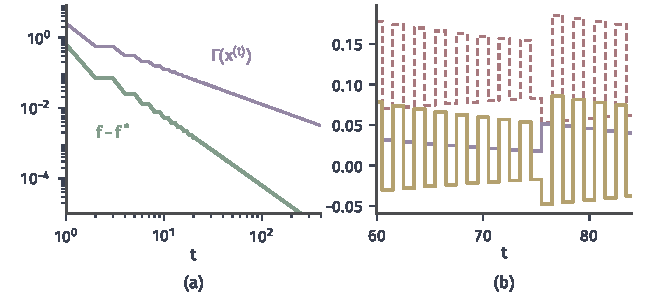
\includegraphics[width=112mm]{figures/05-optimization/06-constrained-optimization/matplotlib/feas-fw-gap-curves/figure.pdf}
  \caption{间隙作为证书，预算例，$\alpha^{(t)}=2/(t+2)$。(a)紫线是$\Gamma(\bm{x}^{(t)})$，绿线是目标差，前者始终在上方。(b)第$60$至$84$轮，内层返回次优顶点时：黄线是算出的$\tilde\Gamma$，紫线是真实间隙$\Gamma$，红色虚线是$\tilde\Gamma+\varepsilon$，$\varepsilon=0.1$。}
  \label{fig:feas-fw-gap-curves}
\end{BookInlineFigure}

\subsection{活跃顶点的调整（补充）}
\label{sec:feas-fw-away}

本小节是补充内容。第~\ref{sec:feas-fw-linear}节留下一个问题：旧顶点的权重只能等比例缩小。如果最优解不用某个顶点，这个顶点的权重永远消不掉，该怎么办？

\paragraph{之字形现象}
用精确线搜索从$\bm{e}_3$出发，第一步$\alpha=\tfrac34$，得到$(0,\tfrac34,\tfrac14)$。第二步$\alpha=\tfrac49$，得到$(\tfrac49,\tfrac{5}{12},\tfrac{5}{36})$。

$\bm{e}_3$的权重每步只乘以$1-\alpha^{(t)}$，线搜索的$\alpha^{(t)}$逐渐变小，第$1000$步第三个坐标仍约为$1.2\times10^{-3}$。图~\ref{fig:feas-fw-away}(a)显示，路径在底边上方反复横跳，既要减小$x_3$，又要调整$x_1,x_2$。这也解释了图~\ref{fig:feas-fw-step-rules}(b)：预定序列的第一步$\alpha^{(0)}=1$恰好把$\bm{e}_3$清零，这个好处只因为起点恰好是要丢弃的顶点，一般问题上不能指望。

\paragraph{远离步}
既然能朝好的顶点走，也应该能从坏的顶点离开。把$\bm{x}$写成活跃顶点集$\bm{S}$上的凸组合，权重$w_{\bm{v}}>0$。\term{远离步}（away step）选出活跃顶点中线性模型最差的一个，沿着背离它的方向走：
\begin{equation}
 \bm{v}^{(t)}\in\argmax_{\bm{v}\in\bm{S}}\langle\bm{g}^{(t)},\bm{v}\rangle,
 \qquad
 \bm{d}=\bm{x}^{(t)}-\bm{v}^{(t)}.
 \label{eq:feas-away}
\end{equation}

新点是$\bm{x}+\gamma\bm{d}$，各权重变成$(1+\gamma)w_{\bm{u}}$，而$\bm{v}^{(t)}$的权重变成$(1+\gamma)w_{\bm{v}}-\gamma$。它必须非负，这给出步长上限
\[
 \gamma\leq\gamma_{\max}=\frac{w_{\bm{v}}}{1-w_{\bm{v}}}.
\]
当$\bm{S}$只有一个顶点时$w_{\bm{v}}=1$，$\gamma_{\max}$无定义，这时不存在远离方向，只走普通的Frank--Wolfe步。取到$\gamma=\gamma_{\max}$时该顶点的权重正好变成零，从活跃集中删除，这称为丢弃步。

\paragraph{成对更新}
另一种做法是把权重直接从最差的活跃顶点搬到最好的顶点。\term{成对步}（pairwise step）取方向$\bm{d}=\bm{s}^{(t)}-\bm{v}^{(t)}$，权重更新是
\[
 w_{\bm{s}}\leftarrow w_{\bm{s}}+\gamma,\qquad
 w_{\bm{v}}\leftarrow w_{\bm{v}}-\gamma,\qquad
 0\leq\gamma\leq w_{\bm{v}}.
\]
其他权重不变，所有权重非负、和为一，所以新点仍是可行的凸组合。

用预算例走一遍，每步用精确线搜索并在上限处截断。第一步只有$\bm{e}_3$活跃，$\bm{s}=\bm{e}_2$，$\gamma=\tfrac34$，到达$(0,\tfrac34,\tfrac14)$。

第二步$\bm{g}=(-1,\tfrac12,\tfrac12)$，$\bm{s}=\bm{e}_1$，$\bm{e}_2,\bm{e}_3$并列最差，取$\bm{v}=\bm{e}_3$。方向$\bm{d}=(1,0,-1)$，精确步长是$1.5/3=\tfrac12$，超过上限$w_{\bm{e}_3}=\tfrac14$，于是截断成丢弃步：
\[
 \bm{x}=\bigl(\tfrac14,\tfrac34,0\bigr).
\]

第三步$\bm{g}=(-\tfrac34,\tfrac12,0)$，$\bm{s}=\bm{e}_1$，$\bm{v}=\bm{e}_2$，方向$(1,-1,0)$，精确步长$\tfrac{5/4}{5}=\tfrac14$，得到
\[
 \bm{x}=\bigl(\tfrac12,\tfrac12,0\bigr).
\]
三步到达最优解，此时$\Gamma=0$。图~\ref{fig:feas-fw-away}对比了这两条路径。

\begin{BookInlineFigure}
  \centering
  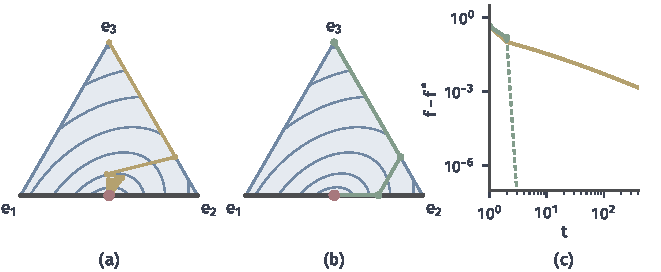
\includegraphics[width=112mm]{figures/05-optimization/06-constrained-optimization/matplotlib/feas-fw-away/figure.pdf}
  \caption{基本流程与成对更新，都用精确线搜索，从$\bm{e}_3$出发。(a)黄色路径是基本的条件梯度法，前$25$步在解上方横跳。(b)绿色路径是成对更新，第二步把$\bm{e}_3$的权重清零，第三步到达解。(c)目标差：黄线是基本流程，绿线是成对更新，第三步目标差为零，虚线表示落到坐标轴下方。}
  \label{fig:feas-fw-away}
\end{BookInlineFigure}

这个三维例子里，到达活动边后问题变成一维二次函数，线搜索一步到位，所以结果格外干净。不能由此推出删除顶点就有线性收敛。这类变体的线性收敛结论依赖目标的曲率、多面体的几何常数（描述顶点相对于面的“尖锐”程度），并要单独计数那些权重被顶到零的步，证明篇幅较长，读者可查阅关于Frank--Wolfe变体线性收敛的专门论文。此外，这些方法要保存活跃顶点及其权重，存储和维护的代价随活跃集增长。
